\vspace{-1cm}
\section{Method}
\noindent The chosen method to answer the research question is to find the optimal dimensions through optimization. Optimization in sports is helpful for finding optima in control and parameters \cite{ackermann_optimality_2010}. The steps that need to be taken to solve the optimization problem are:
\begin{enumerate}
    \item Understanding the Mechanics of the ollie through literature and a video analysis
    \item Optimal control problem and parameter optimization
    \item Implementing the mechanics into the optimization
    \item Solve the optimization problem for the dimensions of the skateboard for maximum ollie height. 
\end{enumerate}

Before I start with the analysis, I will explain all terminology of the parts of the skateboard. All parts are described with figure \ref{f_skateterminology}. The tail is the inclined part with a rounded top. The nose is the mirrored part on the other side of the skateboard. The tail inclination is with respect to the deck. The kink between the deck and the tail or nose is called the pocket. The deck in skateboard terminology is referred to the tail, nose and the part in between. Though, in this paper the deck refers exclusively to the indicated part in figure \ref{f_skateterminology}. Two trucks connect the wheels to the axles with ball bearings. The top of the skateboard is covered with a sandpaper-like sticker called grip-tape (black part). Concave is the radius of the deck. All pictures in this paper will refer to the front as the right hand side of the skateboard and the back as the left hand side. A riding direction is assumed to be positive right. This convention is chosen because left and right are ambiguous in skateboard terminology as the front foot can be either the right or left leg depending on the stance (goofy, regular respectively). 
\begin{figure}[b]
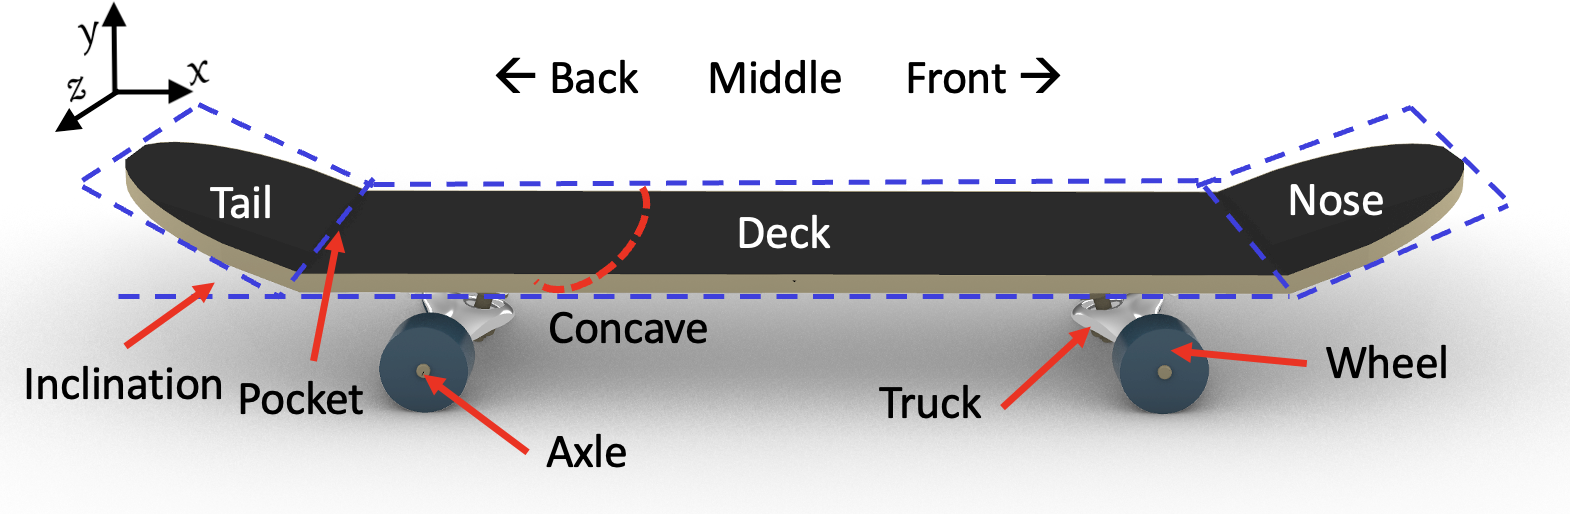
\includegraphics[width=0.5\textwidth]{figure/terminology.png}
\caption[Skateboard terminology]{Skateboard terminology}
\label{f_skateterminology}
\end{figure}
